\chapter{Performance-Analysis}

Before going into performance tests, it is required to understand some fundamentals about network communication and the anatomy of a \gls{http} request.

\section{Introduction}

"To reduce their design complexity, most networks are organized as a \textbf{stack of layers or levels}, each one built upon the one below it" \cite{kn1}[sec. 1.3.1]. The same holds true for the protocol stack driving the "internet". There exist various models for naming and describing the different layers. In context of the internet usually the "TCP/IP Reference Model" is used \cite{kn1}. This model describes five independent layers, each build upon the next underlying layer. 

Real communication between two systems, i.e. exchange of data, always happens on the lowest layer (the "Physical Layer"). But from a logical point of view, communication happens on each layer between the two systems. Therefore each layer might add a header in front of the data, specifying meta information for its counterpart on the other system. Headers of layers above the current layer are treated as plain data, just as the actual message (see figure \ref{fig:header-layers}).

%\begin{wrapfigure}{r}{.45\textwidth}
\begin{figure}[H]
	\centering
	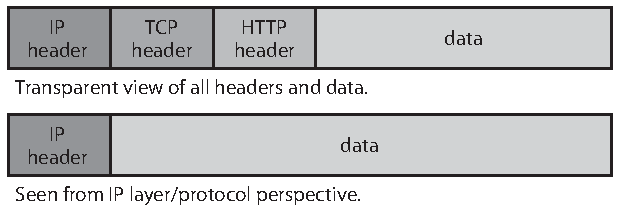
\includegraphics[scale=1]{images/protocol-headers.pdf}
	\caption{Header data for multiple protocol layers.}
	\label{fig:header-layers}
\end{figure}
%\end{wrapfigure}

Figure \ref{fig:net-layers} shows the five layers of the TCP/IP model with corresponding communication protocol and module implementing the protocol on the developed test system. When constructing performance tests this needs to be taken into account to determine for a single parameter which parts of the system are involved and might limit further improvements.

%\begin{wrapfigure}{r}{.5\textwidth}
\begin{figure}[H]
	\centering
	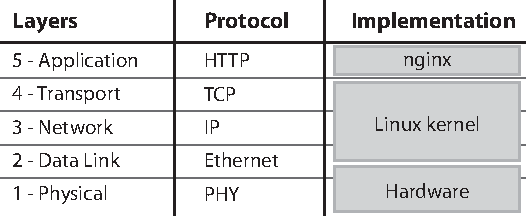
\includegraphics[scale=1]{images/network-layers.pdf}
	\caption{Layers of the network stack with reference to implementing modules.}
	\label{fig:net-layers}
\end{figure}
%\end{wrapfigure}

\subsection{Maximal Transfer Unit (MTU)}
\label{subsec:mtu}

The \gls{mtu} is the maximum size of a single unit transferred over the network in bytes. It is a parameter set for a complete network (sender, receiver, intermediate stations), specifying and limiting its capacity to a robust and reliable usage level. On differing \gls{mtu} values for connected stations the lowest takes effect. In Ethernet networks the \gls{mtu} is usually set to 1500 bytes \cite{kn1}. This includes only the data as received by the Ethernet layer. Header data of  the Ethernet protocol does not count into this size limit. When messages (including header data of upper layers) exceed the \gls{mtu} size, they are split up into multiple packets. In practice this means that for transmitting a single HTTP message (i.e. request or response) two or more \gls{tcp} messages might be required.

\subsection{Transmission Control Protocol (TCP)}

Although \gls{http} is not fixed to be used only with \gls{tcp}; \gls{http} on top of \gls{tcp} on top of \gls{ip} is the most dominant usage combination. This is, because \gls{tcp} provides reliable communication on top of unreliable networks \cite{tcp}. \gls{tcp} accomplishes this by setting up and maintaining a connection. Therefore sending data over TCP consists of three steps: establishing a connection, sending the actual message, closing the connection. To guarantee arrival of sent data, \gls{tcp} works with a handshake protocol between both involved parties. Maintaining a connection is the price to be paid for a reliable communication channel between two systems. But it also allows sending more than one messages using an already established connection. This comes in handy, when a message size exceed the \gls{mtu} or multiple \gls{http} requests are send to a server (used in persistent HTTP connections, also called "HTTP keep-alive" \cite{http}).

\gls{ip} introduced so called IP addresses as identifiers for single systems. \gls{tcp} extends this model by port numbers. An application providing services to other system (i.e. a server) uses one single port, but client applications need to open separate ports for each \gls{tcp} connection. This is required, because \gls{tcp} connections are identified by the four parts "server address", "server port", "client address" and "client port" \cite{tcp}. The TCP header contains two 16 bit fields for source and destination port \cite{kn1}. This leads to a maximum of $2^{16} = 65,536$ concurrently used (open) \gls{tcp} connections on a single client system.

\section{Measuring Web Server Performance}

Network performance is often measured as throughput in bits per second. While this gives a great insight in the capabilities of the network, there is no indication as to how many users can be served concurrently by a web server running on the system under test. To gain insights in this performance parameter, dedicated tests on \gls{http} level need to be performed.

A simple method for measuring request throughput is to "send requests to the server at a fixed rate and to measure the rate at which replies arrive" \cite{httperf}. By monotonically increasing the request rate, the server becomes saturate  at a certain point. This becomes visible in leveling off reply rates and shows that the server operates at full capacity. \cite{httperf}

\subsection{Tools}

\subsubsection{httperf}

\textit{httperf}\footnote{\url{http://www.hpl.hp.com/research/linux/httperf/}} is a tool developed at Hewlett-Packard by David Mosberger and Tai Jin to specifically measure web server performance \cite{httperf}.

\textit{httperf} has three relevant command line arguments for performing the desired performance tests: \texttt{rate}, \texttt{num-conns} and \texttt{num-calls}.

The \texttt{rate} parameter specifies the rate at which connections are created per second. \texttt{num-conns} specifies the total number of connections to be created during one test run. \texttt{num-calls} specifies the number of requests made over a single TCP connection before it is closed.

When executing \textit{httperf} a warning might be displayed:

\texttt{warning: open file limit > FD\_SETSIZE; limiting max. \# of open files to FD\_SETSIZE}

What it basically means is that the current process reached the limit of concurrently allowed open file descriptors. This is a per process limit enforced by the \gls{os}. \textit{httperf} is using the \textit{select}\footnote{"\texttt{select}" is an event library provided by the Linux kernel.} module for dealing with network tasks and creates a new file descriptor for every TCP connection. Therefore the limit on open file descriptors limits the number of TCP connections by \textit{httperf} and therefore might influence conducted performance tests.

To circumvent this issue limits on the current system need to be increased and \textit{httperf} re-compiled. This includes three steps\footnote{The described solution to the FD\_SETSIZE problem was taken from Guillaume Maury: \url{http://gom-jabbar.org/articles/2009/02/04/httperf-and-file-descriptors}.}:

\begin{enumerate}
\item The following line needs to be inserted (or updated) in \texttt{/etc/security/limits.conf}: "\texttt{* hard nofile 65535}". This increases the hard limit of open file descriptors for all users.

\item The value of the pre-compiler constant "\texttt{\_\_FD\_SET\_SIZE} needs to be increased to \texttt{65535}. It is defined in "\texttt{/usr/include/bits/typesizes.h}". (Note: This file might be located in another sub-directory, e.g. "\texttt{/usr/include/x86\_64-linux-gnu/bits/typesizes.h}".)

\item httperf needs to be re-compiled from source:\\
 \\
\texttt{wget} \url{ftp://ftp.hpl.hp.com/pub/httperf/httperf-0.9.0.tar.gz}\\
\texttt{tar xvzf httperf-0.9.0.tar.gz \&\& cd httperf-0.9.0\\
./configure \&\& make\\
sudo make install}
\end{enumerate}

A useful helper for automating test runs with increasing connection rate is \textit{autobench}\footnote{\url{http://www.xenoclast.org/autobench/}}. It is a Perl script acting as a wrapper around \textit{httperf} written by Julian Midgley.

\subsubsection{Custom Scripts}

In addition to accurate engineered test cases using \textit{httperf}, custom scripts were used to simply generate load on the server. A small Windows console application written in \texttt{C\#}, utilizing the \textit{Task Parallel Library}\footnote{\url{http://msdn.microsoft.com/de-de/library/vstudio/dd460717.aspx}} turned out to be the most efficient one with best performance characteristics.

It is also included in the appendix of this report (see \ref{appendix:csharp-load}).

\subsubsection{Wireshark}

\textit{Wireshark}\footnote{\url{http://www.wireshark.org}} is a network protocol analysis software, which captures all traffic going through a network interface. It especially helps in analyzing and inspecting captured data through deep knowledge of all common protocols.

It was used in this project for debugging initial problems with the network stack and low-level analysis of performance  test parameters.


\section{Tests}

The tests were conducted using \textit{httperf} on a virtual machine running \textit{Ubuntu Linux 12.04}. To proof that the limiting factor during the tests is not this client machine, but the system under test, all tests were also performed against a \textit{Microsoft IIS 7.5} web server instance on top of a \textit{Microsoft Windows 7 Professional} operating system running on a bare metal machine with an \textit{AMD Phenom II X4 965} processor at 3.40 GHz.

According to the \textit{HTTP Archive}\footnote{\url{http://httparchive.org/interesting.php\#responsesizes} (as of Dec. 15th 2012)} an average HTML page has a size of about 6 kB. Other content types, like images, stylesheets and script files vary on average between 5 kB and 21 kB. Therefore tests were performed using static files with two sizes: one file having exactly 10 kB (10.240 bytes) from now on referred to as "10K.html" and one very minimal HTML page having just 354 bytes ("index.html"). The major difference between these two files from a "network perspective" is that the small file can be transmitted in two TCP packets (one for the HTTP header and one for the actual data, see section \ref{sec:nginx-os-if}), whereas the 10 KB file needs to be split up in 9 TCP packets due to the default \gls{mtu} size of 1500 bytes.

The following figure (\ref{fig:initial-req}) shows request and response rates two both files with an increasing connection rate (20 conn./s to 120 conn./s, step size: 10). On each connection three HTTP requests were made to the respective file. On every connection rate level 3.000 connections were opened to obtain reliable results.

\begin{figure}[H]
	\centering
	\begin{tikzpicture}
		\begin{axis}[width=\textwidth,height=7cm,
			xlabel={demanded request rate (per second)},
			ylabel={per second},
			extra y tick style={grid=major},
			extra x tick style={grid=major},
			y tick label style={/pgf/number format/1000 sep=},
			ymajorgrids=true,
			legend pos = south east]
			\addplot table[x index=0, y index=1] {graphdata/perf-initial2.csv};
			\addlegendentry{request rate (index.html)}
			\addplot table[x index=0, y index=8] {graphdata/perf-initial2.csv};
			\addlegendentry{reponse rate (index.html)}
			\addplot table[x index=0, y index=2] {graphdata/perf-initial2.csv};
			\addlegendentry{request rate (10K.html)}
			\addplot table[x index=0, y index=9] {graphdata/perf-initial2.csv};
			\addlegendentry{reponse rate (10K.html)}
		\end{axis}
	\end{tikzpicture}
  \caption{Request and response rates for two static files (\texttt{10K.html} and \texttt{index.html}).}
  \label{fig:initial-req}
\end{figure}

The difference between request and response rate origins in failed requests. The following figure shows the corresponding error rate which increases with over-saturating the system.

\begin{figure}[H]
	\centering
	\begin{tikzpicture}
		\begin{axis}[width=\textwidth,height=6cm,
			xlabel={demanded request rate (per second)},
			ylabel={error rate (\%)},
			extra y tick style={grid=major},
			extra x tick style={grid=major},
			y tick label style={/pgf/number format/1000 sep=},
			minor tick style={very thin, gray},
			minor y tick num=3,
			ymajorgrids=true,
			legend pos = north west]
			\addplot table[x index=0, y index=15] {graphdata/perf-initial2.csv};
			\addlegendentry{index.html}
			\addplot table[x index=0, y index=16] {graphdata/perf-initial2.csv};
			\addlegendentry{10K.html}
		\end{axis}
	\end{tikzpicture}
  \caption{Error rate (failed requests) for two static files (\texttt{10K.html} and \texttt{index.html}).}
  \label{fig:initial-req-errors}
\end{figure}

The response \textbf{rate} decreases only slowly with growing saturation, but the average response \textbf{time} increases from  5 ms to about 500-650 ms:

\begin{figure}[H]
	\centering
	\begin{tikzpicture}
		\begin{axis}[width=\textwidth,height=6cm,
			xlabel={demanded request rate (per second)},
			ylabel={response time / ms},
			extra y tick style={grid=major},
			extra x tick style={grid=major},
			y tick label style={/pgf/number format/1000 sep=},
			minor tick style={very thin, gray},
			minor y tick num=3,
			ymajorgrids=true,
			legend pos = south east]
			\addplot table[x index=0, y index=10] {graphdata/perf-initial2.csv};
			\addlegendentry{index.html}
			\addplot table[x index=0, y index=11] {graphdata/perf-initial2.csv};
			\addlegendentry{10K.html}
		\end{axis}
	\end{tikzpicture}
  \caption{Response time for two static files (\texttt{10K.html} and \texttt{index.html}).}
  \label{fig:initial-req-time}
\end{figure}

\begin{wrapfigure}[16]{r}{.5\textwidth}
	\centering
	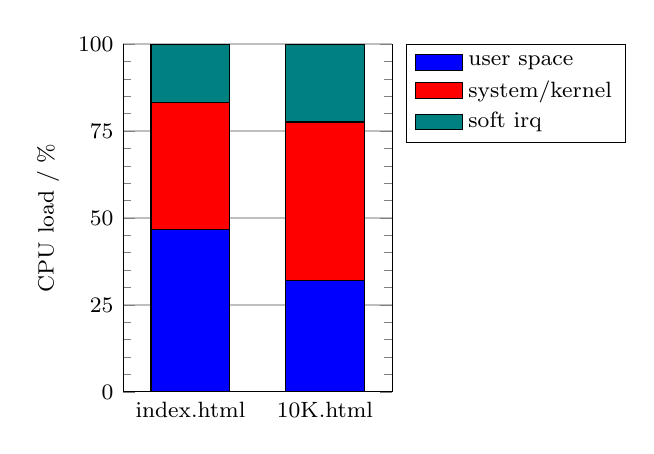
\begin{tikzpicture}
		\begin{axis}[ybar stacked,
			legend style={at={(1.05,1.0)},anchor=north west},
			xtick={0,1},
			axis x line*=bottom,
			tick label style={font=\footnotesize},
			legend style={font=\footnotesize},
			label style={font=\footnotesize},
			ytick={0,25,50,75,100},
			width=5cm,
			height=6cm,
			bar width=10mm,
			ylabel={CPU load / \%},
			xticklabels={index.html, 10K.html},
			ymajorgrids=true,
			minor tick style={very thin, gray},
			minor y tick num=4,
			ymin=0,
			ymax=100,
			area legend,
			legend cell align=left,
			enlarge x limits=0.5]
			\addplot[fill=blue] coordinates % usr
			{(0,46.6) (1,32.1)};
			\addplot[fill=red] coordinates % sys
			{(0,36.5) (1,45.5)};
			\addplot[fill=teal] coordinates % sirq
			{(0,16.7) (1,22.3)};
			\legend{user space,system/kernel,soft irq}
		\end{axis}
	\end{tikzpicture}
	\caption{CPU load distribution for different request types.}
  \label{fig:initial-req-cpu}
\end{wrapfigure}

The difference in request and response rates the system can handle is also visible in \textbf{CPU utilization}. Main responsibility of \textit{nginx} for serving requests is to handle the HTTP part. This includes parsing the request header, generating responses and delivering static files. The \gls{os} on the other hand does the "translation" to and from \gls{tcp} and handles all lower layers (see also figure \ref{fig:net-layers}). An increased payload size of single responses entails therefore a shift in processing time from \textit{nginx} ("user space") to the operations inside the Linux kernel.

The \textbf{network throughput} of both tests follows naturally the trend of response rates. For the test requesting the "index.html" file, the shown throughput is very low, because \textit{httperf} calculates the average throughput as $\cfrac{\text{[size]} \cdot \text{[total repsonses]}}{\text{[test time]}}$.
\vspace{1cm}

\begin{figure}[H]
	\centering
	\begin{tikzpicture}
		\begin{axis}[width=\textwidth,height=6cm,
			xlabel={demanded request rate (per second)},
			ylabel={KB / s},
			extra y tick style={grid=major},
			extra x tick style={grid=major},
			y tick label style={/pgf/number format/1000 sep=},
			minor tick style={very thin, gray},
			minor y tick num=3,
			ymajorgrids=true,
			legend pos = north west]
			\addplot table[x index=0, y index=13] {graphdata/perf-initial2.csv};
			\addlegendentry{index.html}
			\addplot table[x index=0, y index=14] {graphdata/perf-initial2.csv};
			\addlegendentry{10K.html}
		\end{axis}
	\end{tikzpicture}
  \caption{Throughput for two static files (\texttt{10K.html} and \texttt{index.html}).}
  \label{fig:initial-req-io}
\end{figure}

\clearpage
\subsection{Network throughput}

To test the maximal network throughput the server can provide, a test needs to be designed focusing just this parameter to prevent other parts of the system under test to get into the way. A constant high exchange of TCP packets can be achieved by transferring single large files over the network. Therefore a large binary (movie) file with a payload size of 33.4 MB was used for throughput tests.

The following figure (\ref{fig:tcp-io-perf}) shows the network throughput for requests to this file with an increasing connection rate and two requests per connection. The system under test goes into saturation at about 61 Megabits/sec. The figure also shows the total CPU utilization of the tested system.

\begin{figure}[H]
	\centering
	\begin{tikzpicture}
		\begin{axis}[width=\textwidth,height=6cm,
			xlabel={connection rate},
			ylabel={$10^6$ bits/s},
			axis  y  line*=left,
			extra y tick style={grid=major},
			extra x tick style={grid=major},
			y tick label style={/pgf/number format/1000 sep=},
			minor tick style={very thin, gray},
			minor y tick num=3,
			ymajorgrids=true,
			legend style = {at={(0.125,-.1)}, anchor=north}]
			\addplot[color=blue,mark=o] table[x index=0, y index=13] {graphdata/tcp-io-perf.csv};
			\addlegendentry{network throughput}
		\end{axis}
		\begin{axis}[width=\textwidth,height=6cm,
			ylabel={percentage},
			axis  y  line*=right,
			axis  x  line=none,
			extra y tick style={grid=major},
			extra x tick style={grid=major},
			y tick label style={/pgf/number format/1000 sep=},
			minor tick style={very thin, gray},
			minor y tick num=3,
			%ymajorgrids=true,
			legend style = {at={(0.93,-.1)}, anchor=north}]
			\addplot[color=red,mark=x] table[x index=0, y index=9] {graphdata/tcp-io-perf.csv};
			\addlegendentry{cpu load}
		\end{axis}
	\end{tikzpicture}
  \caption{Network throughput and CPU load.}
  \label{fig:tcp-io-perf}
\end{figure}

The following figure (\ref{fig:tcp-io-perf-cpu}) shows the CPU utilization by time spent in the different types of the system. It shows that most time is spent in kernel space and handling interrupt requests by the network driver and sub system. nginx (user space) takes only very low CPU utilization and is not the limiting factor in this test.

%usr	%CPU spent by User space applications		
%sys	%CPU spent by the System (kernel mode)		
%nic	%CPU spent by Low priority user mode (nice)		
%Idle	%CPU which is available (idle)		
%io		%CPU spent by I/O waiting		
%irq	%CPU spent servicing interrupt requests		
%sirq	%CPU spent servicing soft irqs	

\begin{figure}[H]
	\centering
	\begin{tikzpicture}
		\begin{axis}[ybar stacked,width=\textwidth,height=6cm,
			xlabel={connection rate},
			ylabel={percentage},
			extra y tick style={grid=major},
			extra x tick style={grid=major},
			y tick label style={/pgf/number format/1000 sep=},
			minor tick style={very thin, gray},
			minor y tick num=3,
			ymajorgrids=true,
			bar width=10mm,
			area legend,
			legend columns=6,
			legend style = {at={(0.5,1.03)}, anchor=south}]
%			legend pos = south east]
			\addplot[fill=red] table[x index=0, y index=2] {graphdata/tcp-io-perf.csv};	%,mark=x
			\addlegendentry{user space  }
			\addplot[fill=blue] table[x index=0, y index=3] {graphdata/tcp-io-perf.csv};	%,mark=o
			\addlegendentry{system/kernel}
%			\addplot[color=magenta,mark=o] table[x index=0, y index=4] {graphdata/tcp-io-perf.csv};
%			\addlegendentry{low priority (nice)}
%			\addplot table[x index=0, y index=5] {graphdata/tcp-io-perf.csv};
%			\addlegendentry{idle}
%			\addplot[color=orange,mark=triangle] table[x index=0, y index=6] {graphdata/tcp-io-perf.csv};
%			\addlegendentry{io (waiting)}
%			\addplot[color=green,mark=|] table[x index=0, y index=7] {graphdata/tcp-io-perf.csv};
%			\addlegendentry{irq}
			\addplot[fill=teal] table[x index=0, y index=8] {graphdata/tcp-io-perf.csv};	%,mark=diamond
			\addlegendentry{soft irq}
		\end{axis}
	\end{tikzpicture}
  \caption{CPU utilization by category.}
  \label{fig:tcp-io-perf-cpu}
\end{figure}

To proof that obtained performance limits were not limits of the client executing the tests or the network infrastructure, the same test was executed against the "reference system" running an \textit{Microsoft IIS 7.5} web server. Figure \ref{fig:tcp-io-perf-iis} shows the results which outplays the results of the \textit{MicroBlaze} system by more than a factor of eight:

\begin{figure}[H]
	\centering
	\begin{tikzpicture}
		\begin{axis}[width=\textwidth,height=6cm,
			xlabel={connection rate},
			ylabel={$10^6$ bits/s},
			extra y tick style={grid=major},
			extra x tick style={grid=major},
			y tick label style={/pgf/number format/1000 sep=},
			minor tick style={very thin, gray},
			minor y tick num=3,
			ymajorgrids=true,
			legend pos = south east]
			\addplot table[x index=0, y index=15] {graphdata/tcp-io-perf.csv};
			\addlegendentry{network throughput}
		\end{axis}
	\end{tikzpicture}
  \caption{Network throughput of an AMD Phenom II X4 processor at 3.40 GHz running Microsoft IIS 7.5 on Windows 7.}
  \label{fig:tcp-io-perf-iis}
\end{figure}
